%% LyX 2.3.6.1 created this file.  For more info, see http://www.lyx.org/.
%% Do not edit unless you really know what you are doing.
\documentclass[english]{article}
\usepackage[T1]{fontenc}
\usepackage[latin9]{inputenc}
\usepackage{geometry}
\geometry{verbose,tmargin=2.5cm,bmargin=2.5cm,lmargin=2.5cm,rmargin=2.5cm}
\usepackage{graphicx}
\PassOptionsToPackage{normalem}{ulem}
\usepackage{ulem}

\makeatletter

%%%%%%%%%%%%%%%%%%%%%%%%%%%%%% LyX specific LaTeX commands.
%% Because html converters don't know tabularnewline
\providecommand{\tabularnewline}{\\}

\makeatother

\usepackage{babel}
\begin{document}
{[}SPLIT\_HERE{]}
\begin{enumerate}
\item \textbf{{[}DHS/PRELIM/9597/2018/P1/Q1{]} }

A programmer is writing a treasure island game to be played on the
computer. 

The island is a rectangular grid, 30 squares by 10 squares. Each square
of the island is represented by an element in a 2D array. The top
left square of the island is represented by the array element {[}0,
0{]}.

There are 30 squares across and 10 squares down. 

The computer will: 
\begin{itemize}
\item generate three random locations where treasure will be buried 
\item prompt the player for the location of one square where the player
choose to dig
\item display the contents of the array by outputting for each square: 
\begin{itemize}
\item '.' for only sand in this square
\item 'T' for treasure still hidden in sand 
\item 'X' for a hole dug where treasure was found
\item 'O' for a hole dug where no treasure was found. 
\end{itemize}
\end{itemize}
Here is an example display after the player has chosen to dig at location
{[}9, 3{]}: 

\noindent %
\noindent\begin{minipage}[t]{1\columnwidth}%
\texttt{.............................. }

\texttt{.............................. }

\texttt{.............................. }

\texttt{.............................. }

\texttt{..................T........... }

\texttt{.............................. }

\texttt{...T.......................... }

\texttt{.............................. }

\texttt{.............................. }

\texttt{...X..........................}%
\end{minipage}

The game is to be implemented using object oriented programming. 

The programmer has designed the class \texttt{IslandClass}. The identifier
table for this class is: 
\begin{itemize}
\item \texttt{Grid : ARRAY{[}0:9, 0:29{]} OF CHAR} - 2D array to represent
the squares of the island 
\item \texttt{Constructor()} - instantiates an object of class \texttt{IslandClass}
and initialises all squares to sand 
\item \texttt{HideTreasure()} - generates a pair of random numbers used
as the grid location of treasure and marks the square with \texttt{'T'} 
\item \texttt{DigHole(Row, Column)} - takes as parameter a valid grid location
and marks the square with \texttt{'X'} or \texttt{'O'} as appropriate 
\item \texttt{GetSquare(Row, Column) : CHAR} - takes as parameter a valid
grid location and returns the grid value for that square from the
\texttt{IslandClass} object 
\item \texttt{DisplayGrid()} - shows the current grid data. \texttt{DisplayGrid}
should make use of the getter method \texttt{GetSquare} of the \texttt{IslandClass}
class
\end{itemize}

\subsection*{Task 1.1 }

Write program code for the class \texttt{IslandClass} including the
\texttt{Constructor}, \texttt{GetSquare} and \texttt{DisplayGrid}
methods. The code should follow the specification given. 

The value to represent sand should be declared as a constant. Do not
attempt to write the methods \texttt{HideTreasure} or \texttt{DigHole}
at this stage.

\subsection*{Evidence 1}

Program code for Task 1.1\hfill{} {[}5{]}

\subsection*{Task 1.2 }

Write program code for the \texttt{HideTreasure} method. Your method
should check that the random location generated does not already contain
treasure. The value to represent treasure should be declared as a
constant. 

\subsection*{Evidence 2 }

Your program code for Task 1.2\hfill{} {[}3{]}

\subsection*{Task 1.3 }

Write a main program to: 
\begin{itemize}
\item create an IslandClass object 
\item generate three random locations where treasures will be buried
\item your program will then call the DisplayGrid method. 
\end{itemize}

\subsection*{Evidence 3 }

The program code for Task 1.3 \hfill{}{[}3{]}

\subsection*{Evidence 4}

Screenshot showing the output from running the program in Task 1.3\hfill{}
{[}1{]}

\subsection*{Task 1.4 }

Write program code for the \texttt{DigHole} method. This method takes
two integers as parameters. These parameters form a valid grid location.
The location is marked with \texttt{'X'} or \texttt{'O'} as appropriate. 

The values to represent treasure, found treasure and hole should be
declared as constants. 

\subsection*{Evidence 5}

Program code for Task 1.4. \hfill{}{[}3{]}

\subsection*{Task 1.5 }

Add code to the main program in Task 1.3. The program is to: 
\begin{itemize}
\item prompt the player for a location to dig 
\item validate the user input
\item call the \texttt{DigHole} method and then the \texttt{DisplayGrid}
method. 
\end{itemize}

\subsection*{Evidence 6 }

The program code.\hfill{} {[}3{]}

\subsection*{Task 1.6}

Run the program by inputting a location where: 
\begin{itemize}
\item the treasure is not found
\item the treasure is found. 
\end{itemize}

\subsection*{Evidence 7}

Screenshot evidence similar to that shown which shows: 
\begin{itemize}
\item The player has chosen to dig at location {[}2, 25{]} where no treasure
was found 

\noindent\begin{minipage}[t]{1\columnwidth}%
\texttt{.............................. }

\texttt{....T......................... }

\texttt{.........................O.... }

\texttt{..............................}

\texttt{..........T................... }

\texttt{.............................. }

\texttt{..................T........... }

\texttt{.............................. }

\texttt{.............................. }

\texttt{..............................}%
\end{minipage}
\item The player has chosen to dig at location {[}5, 3{]} where treasure
was found 

\noindent\begin{minipage}[t]{1\columnwidth}%
\texttt{.............................. }

\texttt{..............................}

\texttt{...............T..............}

\texttt{.............................. }

\texttt{.........................T.... }

\texttt{...X.......................... }

\texttt{.............................. }

\texttt{..............................}

\texttt{.............................. }

\texttt{..............................}%
\end{minipage}

\hfill{} {[}2{]}
\end{itemize}
{[}SPLIT\_HERE{]}
\item \textbf{{[}DHS/PRELIM/9597/2018/P1/Q2{]} }

The International Bank Account Number (IBAN) is an international bank
account identification standard used in many countries. It uses modulo
arithmetic to perform validation. The IBAN consists of up to 34 alphanumeric
characters, as follows: country code -- two letters check digits
-- two digits, and basic bank account number -- up to 30 alphanumeric
characters that are countryspecific An example of an IBAN in the United
Kingdom Great Britain which is 22 characters is \texttt{GB82WEST12345698765432}
(\texttt{GB} - country code, \texttt{82} - check digits) 

The following is the IBAN check digits generation algorithm: 
\begin{enumerate}
\item[1.]  Initialize the two check digits by \texttt{00} (e.g. \texttt{GB}\texttt{\uline{00}}\texttt{WEST12345698765432}).
\item[2.]  Move the four initial characters to the end of the string (e.g.
\texttt{WEST12345698765432GB}\texttt{\uline{00}}). 
\item[3.]  Replace each alphabet in the string with two digits, using the mapping
A = 10, B = 11, C = 12, . . . . . , Z = 35 (i.e. ASCII value of uppercase
letters - 55) (e.g. \texttt{\uline{32142829}}\texttt{12345698765432}\texttt{\uline{1611}}\texttt{00}). 
\item[4.]  Convert the string to an integer. 
\item[5.]  Calculate the remainder of dividing this number by 97 (e.g. \texttt{3214282912345698765432161100
mod 97 = 16}).
\item[6.]  Subtract the remainder from 98 to give the two check digits (e.g.
check digits \texttt{= 98 - 16 = 82}). If the result is a single digit
number, pad it with a leading 0 to make a two-digit number. 
\end{enumerate}

\subsection*{Task 2.1 }

Write program code for the \texttt{CheckDigits} function using the
following specification. 
\noindent \begin{center}
\texttt{FUNCTION CheckDigits (IBAN : STRING) : STRING }
\par\end{center}

The function has a single string parameter IBAN and returns a two-digit
string result. Use the sample data provided in the text file \texttt{IBANS.txt}
and paste this into your program code.

\subsection*{Evidence 8 }

Your program code. \hfill{}{[}6{]}

\subsection*{Evidence 9 }

One screenshot verifying that your program generates the correct check
digits for the data in \texttt{IBANS.txt}. \hfill{}{[}1{]}

An IBAN is validated by converting it into an integer and performing
a basic mod-97 operation on it. If the IBAN is valid, the remainder
equals 1. The algorithm of IBAN validation is as follows:
\begin{enumerate}
\item[1.]  Move the four initial characters to the end of the string (For the
IBAN \texttt{GB82WEST12345698765432} e.g. \texttt{WEST12345698765432}\texttt{\uline{GB82}}).
\item[2.]  Replace each letter in the string with two digits, thereby expanding
the string, where A = 10, B = 11, C = 12, . . . . . , Z = 35 

(e.g. \texttt{\uline{32142829}}\texttt{12345698765432}\texttt{\uline{1611}}\texttt{82}). 
\item[3.]  Interpret the string as a decimal integer and compute the remainder
of that number on division by 97 

(e.g. \texttt{3214282912345698765432161182 mod 97 = 1}). 
\end{enumerate}
If the remainder is 1, the check digit test is passed and the IBAN
might be valid.

\subsection*{Task 2.2 }

Write a Boolean function \texttt{ValidateIBAN} to determine if a given
IBAN is valid. This function should have a parameter which allows
it to be used for any IBAN. 

\subsection*{Evidence 10 }

Your \texttt{ValidateIBAN} program code. \hfill{}{[}2{]}

\subsection*{Task 2.3 }

A \texttt{TRANSACTIONS.txt} file contains transaction details of customers
of a bank. Each transaction record takes up one line and has three
data fields: customer IBAN, transaction mode (\texttt{W} - withdrawal
or \texttt{D} - deposit) and transaction amount. 

Write a procedure \texttt{CheckIBAN} to read in the IBANs in \texttt{TRANSACTIONS.txt}
and display on the screen: 
\begin{itemize}
\item If an IBAN is valid, the valid IBAN followed by \textquotedblleft \texttt{OK}\textquotedblright . 
\item If an IBAN is invalid, the invalid IBAN followed by \texttt{\textquotedblleft Invalid. Expected
check digits: ??\textquotedblright }, where ?? represents the computed
check digits. 
\item For an invalid IBAN, update the record in \texttt{TRANSACTIONS.txt}
with the expected computed check digits.
\end{itemize}

\subsection*{Evidence 11 }

Your \texttt{CheckIBAN} program code.\hfill{} {[}7{]}

\subsection*{Evidence 12 }

One screenshot showing the output and contents of \texttt{TRANSACTIONS.txt}
from running the program. {[}2{]} 

\subsection*{Task 2.4 }

A master file \texttt{ACCOUNTS.txt} contains the customer IBANs, names
and current balances. 

Write a procedure \texttt{UpdateBalance} to update the current balances
of the customers in \texttt{ACCOUNTS.txt} from \texttt{TRANSACTIONS.txt}.
At the end of the process, your program will output the message: 

\texttt{x records updated. }

\subsection*{Evidence 13}

Your program code for the procedure \texttt{UpdateBalance}.\hfill{}
{[}8{]}

\subsection*{Evidence 14}

One screenshot showing the program output and contents of \texttt{ACCOUNTS.txt}
from running the program.\hfill{} {[}2{]}

{[}SPLIT\_HERE{]}
\item \textbf{{[}DHS/PRELIM/9597/2018/P1/Q3{]} }

A linked list Abstract Data Type (ADT) has the following operations
defined: 
\begin{itemize}
\item \texttt{Create()} -{}- creates an empty linked list; 
\item \texttt{Insert(item, p)} -{}- inserts new value, \texttt{item}, into
linked list so that it is at position \texttt{p} in the linked list.
Assume that the linked list contains at least \texttt{(p - 1)} items
before the insertion. 
\item \texttt{Delete(p)} -{}- deletes the item at position \texttt{p} in
the linked list; 
\item \texttt{Length()} -{}- returns the number of items in the linked list; 
\item \texttt{IsEmpty()} -{}- returns \texttt{True} if linked list is empty; 
\item \texttt{IsFull()} -- returns \texttt{True} if linked list is full; 
\end{itemize}
The linked list is implemented by the use of a collection of nodes
that have two parts: the item data and a pointer to the next item
in the list. In addition there is a \texttt{Start} pointer which points
to the first item in the list. 

The unused nodes are linked and the first unused node is the position
where the next new data item is to be stored. Node removed from the
linked list should be returned to \texttt{NextFree} list.
\begin{center}
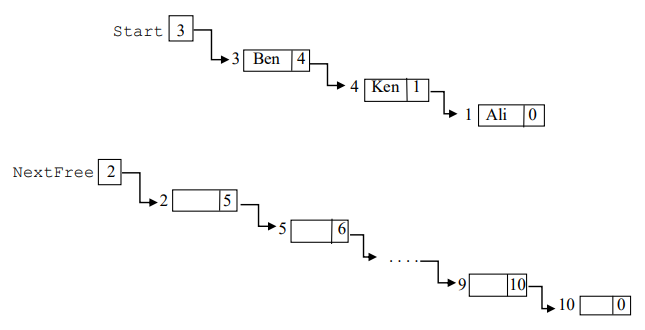
\includegraphics[width=0.65\paperwidth]{static/img/9597-HCI-2018-P1-Q3-1}
\par\end{center}

The diagram shows the linked list after the following sequence of
commands have been executed. 

\noindent\begin{minipage}[t]{1\columnwidth}%
\texttt{Create() }

\texttt{Insert('Ali', 1) }

\texttt{Insert('Jack', 1)}

\texttt{Insert('Ben',2)}

\texttt{Delete(1) }

\texttt{Insert('Jane', 2) }

\texttt{Insert('Ken', 3)}

\texttt{Delete(2)}%
\end{minipage}

The program to implement this ADT will use the classes \texttt{ListNode}
and \texttt{LinkedList} as follows: 
\begin{center}
\begin{tabular}{|l|}
\hline 
\hspace{0.25\columnwidth}\texttt{ListNode}\tabularnewline
\hline 
\texttt{Name : STRING}\tabularnewline
\texttt{Pointer : INTEGER}\tabularnewline
\hline 
\texttt{Constructor()}\tabularnewline
\texttt{SetName(Name:STRING)}\tabularnewline
\texttt{SetPointer(Pointer:INTEGER)}\tabularnewline
\texttt{GetName():STRING}\tabularnewline
\texttt{GetPointer():INTEGER}\tabularnewline
\hline 
\end{tabular}
\par\end{center}

\begin{center}
\begin{tabular}{|l|}
\hline 
\hspace{0.25\columnwidth}\texttt{LinkedList}\tabularnewline
\hline 
\texttt{Node : ARRAY {[}1..10{]} OF ListNode}\tabularnewline
\texttt{Start : INTEGER NextFree : INTEGER}\tabularnewline
\hline 
\texttt{Constructor()}\tabularnewline
\texttt{Insert (name: STRING, position: INTEGER)}\tabularnewline
\texttt{Delete (position: INTEGER)}\tabularnewline
\texttt{Length (): INTEGER}\tabularnewline
\texttt{IsEmpty(): BOOLEAN}\tabularnewline
\texttt{IsFull() : BOOLEAN}\tabularnewline
\hline 
\end{tabular}
\par\end{center}

\subsection*{Task 3.1 }

Write program code to define the classes \texttt{ListNode} and \texttt{LinkedList}. 

\subsection*{Evidence 15}

Program code for the \texttt{ListNode} and \texttt{LinkedList} classes.
\hfill{}{[}18{]}

\subsection*{Task 3.2 }

A method \texttt{Display()} is to be added, which displays the value
of \texttt{Start}, the value of \texttt{NextFree} and the contents
of \texttt{Node} array in index order. Write program code to implement
this method.

\subsection*{Evidence 16}

Your program code for Task 3.2. \hfill{}{[}4{]}

\subsection*{Task 3.3 }

Write code to create a \texttt{LinkedList} object in the main program.
Paste the sequence of commands in \texttt{COMMANDS.txt} into your
program code. Your program will then call the \texttt{Display} method. 

Execute your program to test it.

\subsection*{Evidence 17 }

Screenshot showing the output from running the program in Task 3.3.
\hfill{}{[}2{]}

A linear queue is implemented using the \texttt{LinkedList} class
as a super class. 

The subclass \texttt{Queue} has the following methods: 
\begin{itemize}
\item \texttt{Enqueue(item)} -{}- inserts item at the rear of the queue;
\item \texttt{Dequeue()} -{}- deletes the item at the front of the queue; 
\item \texttt{Display()} -{}- displays the contents of the queue using the
format given below.
\noindent \begin{center}
\texttt{}%
\begin{tabular}{lcl}
\texttt{Steven} & \texttt{$\leftarrow$} & \texttt{Front}\tabularnewline
\texttt{Celine} &  & \tabularnewline
\texttt{Tom} &  & \tabularnewline
\texttt{Ryan} & \texttt{$\leftarrow$} & \texttt{Rear}\tabularnewline
 &  & \tabularnewline
\multicolumn{3}{l}{\texttt{Numbers in queue : 4}}\tabularnewline
\end{tabular}
\par\end{center}
\end{itemize}

\subsection*{Task 3.4 }

Write program code for the subclass \texttt{Queue}.

Use appropriate inheritance and polymorphism in your design. 

\subsection*{Evidence 18}

Your program code for Task 3.4. \hfill{} {[}5{]}

\subsection*{Task 3.5 }

Write program code to: 
\begin{itemize}
\item create a new queue and add the data in the file \texttt{NAMES.txt}
to the queue 
\item remove two items from the queue 
\item display final contents of the queue 
\end{itemize}

\subsection*{Evidence 19 }

Your program code for Task 3.5. \hfill{} {[}2{]}

\subsection*{Evidence 20}

Screenshot showing the output from running the program in Task 3.5.
\hfill{} {[}1{]}

{[}SPLIT\_HERE{]}
\item \textbf{{[}DHS/PRELIM/9597/2018/P1/Q4{]} }

The Romans had their own system of number representation which used
a sequence of upper case letter characters to represent a number.
We shall consider the denary number 1 to 20 only. 

The following letters represent each of the values shown: 
\noindent \begin{center}
\begin{tabular}{|c|c|}
\hline 
Roman Numeral  & Represents\tabularnewline
\hline 
I & One\tabularnewline
\hline 
V & Five\tabularnewline
\hline 
X & Ten\tabularnewline
\hline 
L & Fifty\tabularnewline
\hline 
\end{tabular}
\par\end{center}

A number is always written with the smallest number of characters,
with the letters in sequence starting with the character with the
largest value. 
\begin{itemize}
\item For example, 6 is written \texttt{VI} (not \texttt{IIIIII}) 
\end{itemize}
The exceptions to this sequence are as follows: 
\begin{itemize}
\item one less than 5 -{}- which is written as \texttt{IV}
\item one less than ten -{}- which is written as \texttt{IX} 
\item ten less than fifty -{}- which is written as \texttt{XL} 
\end{itemize}

\subsection*{Task 4.1}

Write program code with the following specification: Input a denary
integer number in the range 1 to 20 Validate the input Calculate the
Roman numeral representation (write this code as a function) Output
the Roman number. 

\subsection*{Evidence 21 }

Your program code. \hfill{}{[}6{]}

\subsection*{Task 4.2 }

Draw up a list of \textbf{three} suitable tests and provide screenshot
evidence for your testing.

\subsection*{Evidence 22 }

Annotated screenshots for each test data run.\hfill{} {[}3{]}

\subsection*{Task 4.3}

Write additional program code with appropriate data validation for
the following specification:
\begin{itemize}
\item Input two Roman numeral numbers between 1 and 20 
\item Ouput the sum of the numbers as a Roman numeral number.
\end{itemize}

\subsection*{Evidence 23 }

Your program code.\hfill{} {[}8{]}

\subsection*{Task 4.4 }

Draw up a list of \textbf{three} suitable tests and provide screenshot
evidence for your testing. 

\subsection*{Evidence 24 }

Annotated screenshots for each test data run. \hfill{}{[}3{]}

{[}SPLIT\_HERE{]}
\item \textbf{{[}DHS/PRELIM/9597/2018/P2/Q1{]} }
\begin{enumerate}
\item A local area network can be set up as either client-server or peer-to-peer.
\begin{enumerate}
\item State where data are stored on a client-server network and why? \hfill{}{[}1{]}
\item State where data are stored on a peer-to-peer network and why? \hfill{}{[}1{]}
\item In your opinion, what is the key benefit of a client-server network
over peer-topeer network. Justify. \hfill{}{[}2{]}
\item In your opinion, what is the main drawback of a client-server network
compared to a peer-to-peer network. Justify. \hfill{}{[}2{]}
\end{enumerate}
\item A 60 Megabyte file is transferred over a network to a printer in 10
seconds. 

Calculate the transfer rate, in kilobytes per second, used to transfer
this file. Show all of your working. {[}1 MB = 1024 KB{]} \hfill{}{[}2{]}
\item Explain how DHCP operates in a network? \hfill{}{[}3{]}
\item Switches and routers are both connecting devices.
\begin{enumerate}
\item What are the purposes of having connecting device in a network?\hfill{}
{[}2{]}
\item What are the differences between them?\hfill{} {[}2{]}
\end{enumerate}
\end{enumerate}
{[}SPLIT\_HERE{]}
\item \textbf{{[}DHS/PRELIM/9597/2018/P2/Q2{]} }
\begin{enumerate}
\item What are the characteristics of a voice-user interface? \hfill{}{[}2{]}
\item What are the strengths and weaknesses of a voice-user interface in
comparison to a graphical user-interface?\hfill{}{[}4{]}
\item One of the 8 golden rules for interface design is the element of consistency. 
\begin{enumerate}
\item Explain the importance of consistency in designing a user interface.
\hfill{}{[}4{]}
\item Is consistency still important in the newer user-interfaces (eg. voice,
gesture)? Why is this so?\hfill{} {[}2{]}
\item Voice User interfaces gaining popularity with the readily availablity
of devices like Echo and iphone. What do you think are some of the
key design elements that are vital to an effective user experience
when using such devices? Explain your answers.\hfill{} {[}3{]}
\end{enumerate}
\end{enumerate}
{[}SPLIT\_HERE{]}
\item \textbf{{[}DHS/PRELIM/9597/2018/P2/Q3{]} }
\begin{enumerate}
\item Explain what is meant by the following terms and give an example for
each
\begin{enumerate}
\item Candidate key\hfill{} {[}2{]}
\item Secondary key \hfill{} {[}2{]}
\item Foreign key\hfill{} {[}2{]}
\end{enumerate}
\item The school\textquoteright s Robotics club is looking at designing
a relational database to keep track of members participation and achievements.
Proposed a relational database design for this purpose.
\begin{enumerate}
\item Give the table descriptions in shorthand notations. Explain the purpose
of all your tables. Highlight the necessary details needed in your
design.\hfill{} {[}6{]}
\item Draw the entity-relationship model for your design.\hfill{} {[}3{]}
\end{enumerate}
\end{enumerate}
{[}SPLIT\_HERE{]}
\item \textbf{{[}DHS/PRELIM/9597/2018/P2/Q4{]} }

An apartment block in a city consists of a large number of apartments.
Each of the residents of the apartments has their information stored
in a file. 

The records in the file are to be sorted into alphabetical order of
the resident\textquoteright s name.
\begin{enumerate}
\item Using the following list of names as an example, show how the records
can be sorted into alphabetical order using an insertion sort. 

GRA, CHR, DAV, SAR, TOM, KAT \hfill{}{[}4{]}
\item Residents sometimes make requests for maintenance on their apartments.
Each request is given a priority number ranging from 1, for failure
of the air conditioning, to 10, for a dripping tap. Each request is
stored in a linked list in order of priorities. Jobs with equal priority
are stored in order of the date that they have been submitted. 

Describe an algorithm to insert a new job into the list.\hfill{}
{[}6{]}
\end{enumerate}
{[}SPLIT\_HERE{]}
\item \textbf{{[}DHS/PRELIM/9597/2018/P2/Q5{]} }
\begin{enumerate}
\item Explain the difference between an iterative solution and a recursive
solution to a problem. \hfill{}{[}2{]}
\item The program \texttt{RADIX\_CONVERT}, listed below, calls a recursive
procedure, OUT. Note that x DIV y gives the integral part of the quotient
when x is divided by y, and x MOD y gives the remainder. 

\noindent\begin{minipage}[t]{1\columnwidth}%
\texttt{Program RADIX\_CONVERT }

\texttt{\qquad{}declare integers a, b}

\texttt{\qquad{}input a, b OUT (a, b) }

\texttt{\qquad{}print a, b }

\texttt{End RADIX\_CONVERT }

\bigskip{}

\texttt{Procedure OUT (x, y) }

\texttt{\qquad{}declare integers a, b }

\texttt{\qquad{}a = x DIV y }

\texttt{\qquad{}b = x MOD y }

\texttt{\qquad{}if a > 0 then OUT (a, y) }

\texttt{\qquad{}print (b) }

\texttt{End OUT }%
\end{minipage}
\begin{enumerate}
\item Draw a diagram to trace the execution of the program, \texttt{RADIX\_CONVERT}
with values 46 and 3 as input for \texttt{a} and \texttt{b} respectively.
Show clearly the order of call and return, and the change in values
of a and b.\hfill{}{[}4{]}
\item Write down, in the correct order, all the values printed. \hfill{}{[}2{]}
\item What does \texttt{RADIX\_CONVERT} accomplish? \hfill{}{[}2{]}
\end{enumerate}
\end{enumerate}
{[}SPLIT\_HERE{]}
\item \textbf{{[}DHS/PRELIM/9597/2018/P2/Q6{]} }

Carrie Car, a car accessories shop wants to sell its products through
the internet. A software house has been engaged to supply the computerised
solution. The project manager has drawn up a list of activities and
their likely duration. 
\noindent \begin{center}
\begin{tabular}{|c|c|c|}
\hline 
Activity & Description & Weeks to complete\tabularnewline
\hline 
A & Write requirement specification & 5\tabularnewline
\hline 
B & Produce program design & 5\tabularnewline
\hline 
C & Write module code & 15\tabularnewline
\hline 
D & Module testing & 10\tabularnewline
\hline 
E & Integration testing & 5 \tabularnewline
\hline 
F & Alpha testing & 3\tabularnewline
\hline 
G & Install software and acceptance testing & 5\tabularnewline
\hline 
H & Write end user training guide & 5\tabularnewline
\hline 
J & Write technical documentation & 10\tabularnewline
\hline 
K & End user training & 4\tabularnewline
\hline 
L & Sign off final system & 1\tabularnewline
\hline 
\end{tabular}
\par\end{center}
\begin{enumerate}
\item The project manager decides to construct a Program Evaluation Review
Technique (PERT) chart from this data.
\begin{center}
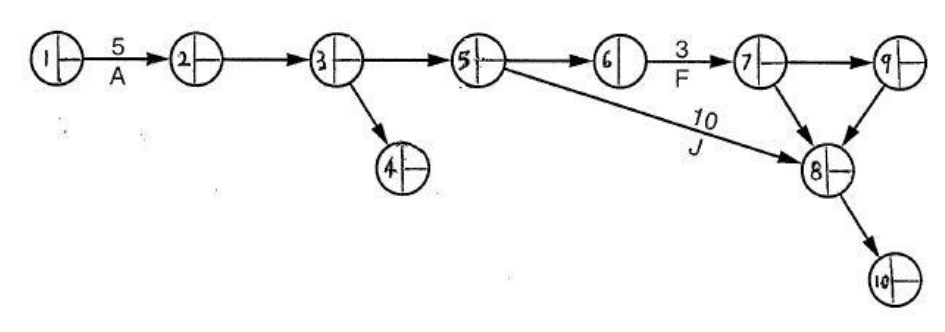
\includegraphics[width=0.5\paperwidth]{static/img/9597-HCI-2018-P2-Q6}
\par\end{center}
\begin{enumerate}
\item Complete the PERT chart. \hfill{}{[}3{]}
\item State the critical path and elapsed time for this project. \hfill{}{[}2{]}
\item State the earliest and late start for activity J. \hfill{}{[}2{]}
\end{enumerate}
\item The systems analyst from the team gathered the following requirements: 
\begin{itemize}
\item A customer can place an order either by telephone or via the internet
\item The order will be placed in a file to be dealt with by the warehouse
staff 
\item An email acknowledgement of the order will be sent to the customer 
\item After completion of the order the customer details will be stored
in a customer file 
\end{itemize}
List details of the data stores required, and draw the data flow diagram
for the solution.\hfill{} {[}6{]}
\item Various procedures are written. One of the procedures is written to
look up the customer record in the customer file. The procedure then
adds the value of the current order to the total ordered by the customer
this year. This determines whether or not a discount is payable. 

Parameters can be passed to a procedure by using pass-by-value or
pass-by-reference. Explain the two methods and highlight the difference.
Using the scenario above, give an example of each to illustrate the
difference. \hfill{}{[}6{]}
\item Besides car accessories, Carrie Car also sells car insurance. Customers
can insure their car using one of two methods: 
\begin{itemize}
\item Method A: by using the Internet or 
\item Method B: by using the telephone to talk to a sales representative. 
\end{itemize}
\begin{enumerate}
\item For method A, describe how the car registration could be validated.
\hfill{}{[}1{]}
\item For method B, describe how the car registration could be verified.
\hfill{}{[}1{]}
\item Explain the difference between data validation and data verification.
\hfill{}{[}2{]}
\end{enumerate}
\item The rules that are used when deciding whether to offer insurance to
customers and whether to offer discounts are as follows:
\begin{itemize}
\item If the customer has been refused insurance by another company and
their car is over 10 years old then insurance is refused.
\item If the customer has been refused insurance by another company and
their car is not more than 10 years old then insurance without any
discount is available. 
\item If the customer has not been refused insurance by another company
and their car is over 10 years old then insurance without any discount
is available. 
\item If the customer has not been refused insurance by another company
and their car is less than 10 years old and they have made not more
than three claims previously then insurance with a discount is available.
\begin{enumerate}
\item Create a decision table showing all the possible outcomes and results. 
\item Simplify your decision table by removing redundancies. \hfill{}{[}7{]}
\end{enumerate}
\end{itemize}
{[}SPLIT\_HERE{]}
\end{enumerate}
\item \textbf{{[}DHS/PRELIM/9597/2018/P2/Q7{]} }

The elements of an array are numbered 0 to MAX. It is wished to copy
all the data items stored in that part of the array between START
and FINISH to a different position in the array, the item at START
moving to NEWSTART.

Describe in detail an algorithm to accomplish this. You may assume
that no items will be moved beyond the range of the array, but remember
that the copying may be in either direction, and that the new position
may overlap the old. \hfill{}{[}5{]}

{[}SPLIT\_HERE{]}
\end{enumerate}

\end{document}
